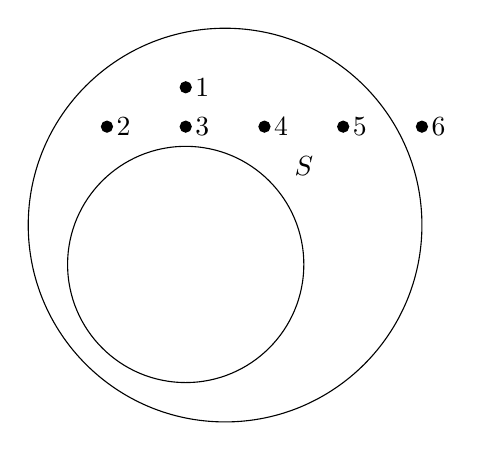
\begin{tikzpicture}[scale=1]
	\draw (0,0) circle (2.5cm);
	\node at (-2.25,2) {$\N$};
	\draw (-.5,-.5) circle (1.5cm);
	\filldraw (-.5,1.75) circle (2pt) node[right] {$1$};
	\foreach \x in {2,3,4,5,6}
	\filldraw (-.5+\x-3,1.25) circle (2pt) node[right] {\x};
	\node at (1,.75) {$S$};
%	\filldraw[blue] (0,1.5) circle (2pt) node[right] {$\min(\N\setminus S)=m>1$};
\end{tikzpicture}